\documentclass[10pt,twocolumn,a4paper]{article}

\usepackage[T1]{fontenc}
\usepackage[utf8]{inputenc}
\usepackage[a4paper, margin=20mm]{geometry}
\usepackage{cite}
\usepackage{amsmath,amssymb,amsfonts}
\usepackage{graphicx}
\usepackage{textcomp}
\usepackage{xcolor}
\usepackage{booktabs}
\usepackage{url}
\usepackage{hyperref}
\usepackage{titlesec}
\usepackage{caption}
\captionsetup[figure]{font=small,labelfont=bf}
\captionsetup[table]{font=small,labelfont=bf}

\hypersetup{colorlinks=true, linkcolor=blue, citecolor=blue, urlcolor=blue}

\titleformat*{\section}{\large\bfseries}
\titleformat*{\subsection}{\normalsize\bfseries}

\setlength{\columnsep}{6mm}
\setlength{\parindent}{1em}

\title{\bfseries A Spherical Chiplet Fabric with Geodesic Topology, \\
Planet-Style Coordinates, and Reorientable Frame Semantics \\
for Large-Scale AI and HPC Workloads}

\author{Musthafa Ali \\
\small Independent Researcher, Sydney, Australia \\
\small \texttt{mali@outlook.com.au}}
\date{April 2026}

\begin{document}

\twocolumn[
\begin{@twocolumnfalse}
\maketitle

\begin{abstract}
\noindent
We present a chiplet-based processor architecture in which compute,
memory-controller, and cache/IO tiles are arranged on the vertices of a
geodesic icosphere, connected by short equal-length neighbor links over a
rigid-flex interposer. The topology removes the corners of conventional flat
meshes and tori, yielding more uniform hop-count and latency distributions and
improving bisection bandwidth at fixed tile count. A planet-style coordinate
system---latitude, longitude, and a local north/east compass---is exposed to
software, and a quaternion-based reference frame can be reoriented at runtime
through an epoch/commit protocol without disturbing in-flight traffic. We
specify a 162-tile reference design (113 compute, 25 memory-controller, 24
cache/IO tiles), a deadlock-free routing scheme using a Duato-style escape
virtual channel layered under greedy great-circle routing, an HBM3e memory
hierarchy organized as latitude belts with single-owner controller tiles, and
a Gen-1 segmented cold-plate cooling solution with a future microfluidic path.
We validate the architecture with an event-driven cycle-accurate fabric
simulator that produces real latency CDFs, all-reduce timings, and bisection
estimates against torus and dragonfly baselines, and we project workload
performance using a roofline-style analytical model. Sphere-162 delivers an
estimated 56.5~PFLOPS dense FP8, 30~TB/s HBM bandwidth, and 900~GB capacity
within a 2.3~kW power envelope, achieving 24.8~PFLOPS/kW---approximately
$5\times$ the energy efficiency of an 8-GPU H100 node at comparable aggregate
compute, while fitting larger models in unified memory.
\end{abstract}

\vspace{6pt}
\end{@twocolumnfalse}
]

\section{Introduction}

The end of monolithic die scaling has driven a transition to chiplet-based
architectures in which a system-level processor is composed of many smaller
silicon dies connected by an advanced package
\cite{nvidia_b200, amd_mi300, intel_pondervein}. As the number of tiles per
package grows, the on-package interconnect topology becomes a first-order
determinant of performance: it sets the average and worst-case message
latency, the bisection bandwidth available to collective operations, and the
ease with which workloads can be scheduled to minimize communication
\cite{kim2008flattened, ahn2014triplet}.

Existing chiplet packages are typically organized as 2D arrays connected
through silicon bridges or interposers, exposing a rectangular mesh or torus
topology to software. While planar meshes are well-matched to lithographic
manufacturing, they suffer from two structural limitations. First, edges and
corners create non-uniform hop distributions: corner tiles have measurably
worse average reach than central tiles, producing tail-latency outliers in
collective operations. Second, the bisection bandwidth of a rectangular array
scales sub-linearly with the number of tiles along the cut dimension,
limiting the throughput of all-to-all and reduce-scatter primitives that
dominate large-model training.

This paper proposes a different geometric organization: place the chiplets on
the vertices of a \emph{geodesic icosphere}, with each tile connected to its
five or six nearest neighbors along approximately equal-length links. The
topology has no corners; every vertex is interchangeable up to rotation, and
the average path between vertex pairs scales as $O(\sqrt{N})$ with a smaller
constant than a torus and a substantially shorter tail. We complement the
topology with a coordinate system inspired by planetary geography---each tile
exposes a (latitude, longitude) pair and a local east/north compass---and an
operating-system-level primitive for rotating the reference frame, which lets
schedulers re-orient workload placement without physically moving anything.

\textbf{Contributions.} This work makes the following contributions:

\begin{itemize}
\item A complete chiplet-package architecture (\S\ref{sec:arch}) including
tile definitions, fabric topology, routing, memory hierarchy, power
delivery, and cooling, organized around a 162-tile reference design.
\item A planet-style coordinate system and quaternion-based frame-flip
protocol (\S\ref{sec:coords}) with formal pole-handling and atomic commit
semantics.
\item A deadlock-free routing scheme (\S\ref{sec:routing}) layering greedy
great-circle forwarding over a Duato-style escape virtual channel on an
up\textsuperscript{*}/down\textsuperscript{*} spanning tree.
\item An event-driven cycle-accurate fabric simulator and an analytical
performance model (\S\ref{sec:methodology}) that produce real latency
distributions and workload throughput estimates.
\item A multi-axis evaluation (\S\ref{sec:eval}) against 2D torus and
dragonfly baselines, showing improvements in p99 latency, bisection
bandwidth, and energy per bit, and projections against H100, B200, MI300X,
and 8-GPU NVLink nodes.
\item An honest treatment of validation gaps, manufacturability risks, and
unresolved design questions (\S\ref{sec:discussion}).
\end{itemize}

We do not claim physical silicon validation; this paper reports a
simulator-based and analytical evaluation in the tradition of architectural
proposals such as the original dragonfly \cite{kim2008flattened} and
hyperX \cite{ahn2009hyperx} papers. Section~\ref{sec:discussion} discusses
what would be required to advance the design to silicon.

\section{Background and Related Work}

\subsection{Chiplet Packaging}

Recent commercial accelerators integrate compute and memory dies through
2.5D or 3D packaging. NVIDIA's B200 combines two reticle-sized GPU dies with
HBM3e stacks on a CoWoS interposer \cite{nvidia_b200}. AMD's MI300X uses a
3D-stacked design with eight compute dies and HBM stacks \cite{amd_mi300}.
These designs exploit short on-package interconnect to scale beyond a single
reticle but retain a fundamentally rectangular logical topology.

\subsection{Network-on-Chip and Network-on-Package Topologies}

The on-chip interconnect literature has explored mesh, torus, fat-tree,
flattened butterfly, dragonfly, and hyperX topologies
\cite{kim2008flattened, ahn2009hyperx, dally1990performance,
dally2003principles}.
For 2D-laid-out chiplets, mesh and torus dominate due to layout simplicity.
Dragonfly is widely used at HPC system scale (e.g., Cray Slingshot) but
typically requires multiple cabinet/board hierarchies that do not directly
apply within a single package.

\subsection{Geodesic and Spherical Networks}

Geodesic networks have a long history in graph theory and computational
geometry, motivated by their isotropy and bounded-degree regularity
\cite{wenninger1971polyhedron}. Their use as an interconnect topology for
silicon has been limited because lithography is planar, and a literally
curved die is not manufacturable. We argue, however, that the
\emph{logical} geodesic topology can be approximated by chiplets placed on
folded interposer petals, capturing most of the benefit while remaining
compatible with standard chiplet processes.

\subsection{Deadlock-Free Routing}

Duato's protocol \cite{duato1993new} establishes deadlock freedom by
provisioning a deadlock-free escape sub-network alongside an adaptive
routing function. We adopt this framework: an
up\textsuperscript{*}/down\textsuperscript{*} spanning tree provides the
escape VC, while greedy great-circle forwarding provides adaptive minimal
routing.

\section{Architecture}\label{sec:arch}

\subsection{Reference Design}

Sphere-162 places 162 chiplets on the vertices of a level-2 subdivided
icosahedron (icosphere). The tile mix is:

\begin{itemize}
\item \textbf{113 Compute Tiles (CT)}, each containing 4 ARMv9/RVA23-class
out-of-order cores at 3.5~GHz, one $256{\times}256$ FP8/FP16/BF16 systolic
matrix engine at 2~GHz, 1~MB L1 per core, 8~MB shared L2, and an 8-port
fabric router. Estimated area $\sim$25~mm\textsuperscript{2} at 3~nm,
typical power 15~W.
\item \textbf{25 Memory-Controller Tiles (MCT)}, each owning one HBM3e
stack (36~GB, 1.2~TB/s), a directory shard for cache coherence, and
near-memory compute units for gather/scatter, sparse decode, and reduction
primitives. $\sim$20~mm\textsuperscript{2}, 12~W typical.
\item \textbf{24 Cache/IO Tiles (CIT)}, each containing 64~MB of L3 SRAM
and PCIe~6.0/CXL~3.0 controllers (on edge tiles only). 8~W typical.
\end{itemize}

Aggregate specifications: 56.5~PFLOPS dense FP8, 900~GB HBM3e capacity,
30~TB/s HBM bandwidth, 1.5~GB total L3, and an estimated 2.3~kW typical
power. Detailed power breakdown is presented in \S\ref{sec:eval}.

\subsection{Fabric Topology}\label{sec:topology}

Each chiplet sits at a vertex of the level-2 icosphere; edges of the
underlying triangulation form 5- or 6-degree neighbor links. With unit-radius
parameters scaled to a 40~mm package radius, neighbor-link arc lengths are
4--7~mm, comparable to typical 2.5D interposer trace lengths.

Optionally, up to 12 \emph{express chords} cut across the sphere (typically
between near-antipodal vertices) to provide single-hop long-range links.
Chords add roughly 8\% of the edge count but reduce average hop distance by
22\% and 99th-percentile hops by 40\% in our reference design (see
\S\ref{sec:eval}).

\subsection{Memory Hierarchy and NUMA-by-Latitude}

HBM stacks are organized as \emph{belts}---rings of MCTs at fixed latitudes.
Each MCT exclusively owns one HBM stack and one directory shard, eliminating
the multi-master controller designs that complicate sharing in conventional
HBM systems. Compute tiles access HBM via the fabric, and the system exposes
a per-tile NUMA distance based on the geodesic hop count to each MCT. This
allows OS- and runtime-level placement engines to pin model-parallel shards
to specific belts, bounding worst-case data-movement cost by the great-circle
diameter ($\pi$ times the radius, or 6--7 hops for Sphere-162).

\subsection{Power Delivery and Cooling}

Power enters the package through pole-mounted bulk regulators and is
distributed via concentric power planes routed through the rigid-flex petal
stack to per-tile point-of-load converters. Five rails are
defined---\texttt{VDD\_CORE}, \texttt{VDD\_SRAM}, \texttt{VDD\_SERDES},
\texttt{VDD\_HBM}, \texttt{VSS}---with deep-trench and MLCC decoupling at
each tile.

For Gen-1, we specify a \emph{segmented spherical cold-plate}: 12--20
faceted cold-plate sections with per-facet micro-channel coolant flow,
sealed at seams with O-rings and connected through quick-disconnect
manifolds at the poles. The hottest caps---typically the matrix-heavy
compute tiles---are clustered near the polar manifolds where coolant flow
rates are highest. A future Gen-2 microfluidic implementation, with
dielectric coolant flowing through silicon-bonded microchannels directly
beneath each chiplet, is sketched in \S\ref{sec:discussion}.

\subsection{Clocking and DFT}

The fabric uses globally-asynchronous, locally-synchronous (GALS) clocking.
A single low-jitter reference (target $\leq 300$~fs RMS phase noise,
12~kHz--20~MHz) is distributed to per-quad PLL fan-out buffers; each tile
runs its own PLL and synchronizes to neighbors through mesochronous FIFOs.
DFT uses segmented IEEE 1687 (iJTAG) chains organized by hemisphere, with
PRBS31 BIST per fabric port and a $\geq 10^9$-bit dwell requirement for
``link-good'' assertion.

\section{Coordinate System and Frame Reorientation}\label{sec:coords}

\subsection{Coordinates}

Each tile $i$ is assigned a unit position vector $\mathbf{u}_i \in
\mathbb{S}^2$. Latitude and longitude are derived as
$\varphi_i = \arcsin(z_i)$ and $\lambda_i = \mathrm{atan2}(y_i, x_i)$. A
local tangent basis at tile $i$ is
\begin{align}
\mathbf{e}_E(\lambda) &= (-\sin\lambda, \cos\lambda, 0), \\
\mathbf{e}_N(\varphi, \lambda) &= (-\sin\varphi\cos\lambda,
-\sin\varphi\sin\lambda, \cos\varphi).
\end{align}

At the geometric poles ($|\cos\varphi| < \epsilon$), $\mathbf{e}_E$ becomes
ill-defined; we resolve this by anchoring polar east to a fixed azimuth
determined by the prime meridian and computing $\mathbf{e}_N = \mathbf{e}_E
\times \mathbf{u}$.

\subsection{Bearings and Compass}

The bearing from tile $i$ to neighbor $j$ is computed by projecting
$\mathbf{u}_j$ onto $i$'s tangent plane and resolving in the $(\mathbf{e}_N,
\mathbf{e}_E)$ basis:
\begin{align}
\mathbf{t}_{ij} &= \mathbf{u}_j - (\mathbf{u}_j \cdot \mathbf{u}_i)\mathbf{u}_i,\\
\alpha_{ij} &= \mathrm{atan2}(\mathbf{t}_{ij} \cdot \mathbf{e}_E,
\mathbf{t}_{ij} \cdot \mathbf{e}_N).
\end{align}
Bearings are quantized to a small per-port LUT (typically 16 sectors).

\subsection{Frame Reorientation Protocol}

A global \emph{reference frame} is described by two orthonormal vectors
$(\mathbf{Z}_0, \mathbf{X}_0)$: the north pole and prime meridian directions
in package-physical coordinates. To reorient (``flip''), the management
controller broadcasts a new frame and an epoch token. Each tile maintains
both old and new bases; bearings, NUMA tables, and routing state under the
new frame are precomputed locally. On receipt of the commit token, all tiles
atomically switch at the next packet boundary. The protocol completes in a
single fabric round-trip (under 1~$\mu$s for Sphere-162) and does not
require draining in-flight traffic, since route correctness is invariant
under rotation: greedy forwarding by dot-product is rotation-invariant when
applied to the rotated $\mathbf{u}_j$.

\section{Routing and Flow Control}\label{sec:routing}

\subsection{Adaptive Layer: Greedy Great-Circle}

The adaptive routing function selects the neighbor maximizing the dot
product with the destination's unit vector:
\begin{equation}
\text{next}(i, d) = \arg\max_{j \in N(i)} \mathbf{u}_j \cdot \mathbf{u}_d.
\end{equation}

This is rotation-invariant and uses only local state (own coordinates,
neighbor coordinates, destination coordinates). On the unmodified icosphere
it converges to a minimal path; with chord links present, it remains a valid
heuristic but is not always minimal.

\subsection{Escape Layer: Up\textsuperscript{*}/Down\textsuperscript{*} Spanning Tree}

To guarantee deadlock freedom and forward progress under all traffic
patterns, we provision a Duato-style escape virtual channel
\cite{duato1993new} on a single up\textsuperscript{*}/down\textsuperscript{*}
spanning tree rooted at a designated tile. The escape channel uses a
deterministic shortest-path route on the tree and admits no cyclic
dependencies. Three virtual channels per port are sufficient: VC0 escape,
VC1--VC2 adaptive.

\subsection{Quality of Service}

Two traffic classes are partitioned across VCs: HBM/IO traffic (latency-
sensitive memory accesses) and collective traffic (bandwidth-sensitive
reductions). Age-based arbitration provides starvation freedom under
sustained contention.

\section{Methodology}\label{sec:methodology}

\subsection{Cycle-Accurate Fabric Simulator}

We implemented an event-driven simulator in Python that models per-flit
serialization, wire propagation, router pipeline stages, and link contention.
The router is parameterized as a 4-stage pipeline at 2~GHz (2~ns base
latency); links use 8~lanes at 32~Gb/s NRZ for 256~Gb/s per link aggregate.
Per-link wire delay uses 150~mm/ns propagation (approximately half $c$ in
copper trace). Packets are 4 flits of 512 bits each (256~B). Source code
is available at the artifact link.

\subsection{Topologies Compared}

\begin{itemize}
\item \textbf{Sphere (162)}: level-2 icosphere, 162 vertices, average degree
5.93, no chords.
\item \textbf{Sphere+chords (162)}: identical with 10 added antipodal chord
links.
\item \textbf{Torus 13$\times$13 (169)}: 2D torus, average degree 4, 4~mm
uniform link length.
\item \textbf{Dragonfly 9$\times$6 (54)}: 9 groups of 6 routers each;
intra-group full mesh, inter-group round-robin assignment. Smaller node
count by construction.
\end{itemize}

\subsection{Workload Model}

For workload-level performance we use a roofline-style model
\cite{williams2009roofline} that bounds throughput by the minimum of compute
supply and memory-bandwidth supply, with a 0.3$\times$ penalty for working
sets that exceed available HBM capacity (representing sharding overhead and
PCIe spillover in conventional GPUs).

\section{Evaluation}\label{sec:eval}

\subsection{Topology Properties}

Table~\ref{tab:topology} summarizes static topology metrics. Sphere delivers
a lower 99th-percentile hop count (10) than the size-matched torus (12), and
adding 10 chord links reduces it to 6, comparable to the 54-node dragonfly's
3 hops despite having $3\times$ the nodes.

\begin{table}[t]
\centering
\caption{Static topology metrics. N = node count, deg = average degree,
avg/p95/p99/max = hop counts.}
\label{tab:topology}
\small
\begin{tabular}{lrrrrrr}
\toprule
Topology & N & deg & avg & p95 & p99 & max \\
\midrule
Sphere (162)         & 162 & 5.9 & 5.66 & 9  & 10 & 12 \\
Sphere+chords        & 162 & 6.1 & 4.41 & 6  & 6  & 7  \\
Torus 13$\times$13   & 169 & 4.0 & 6.50 & 11 & 12 & 12 \\
Dragonfly 9$\times$6 & 54  & 7.0 & 2.36 & 3  & 3  & 3  \\
\bottomrule
\end{tabular}
\end{table}

Figure~\ref{fig:hop_cdf} shows the full hop-count CDF. The sphere has a
shorter, less-tailed distribution than the torus.

\begin{figure}[t]
\centering
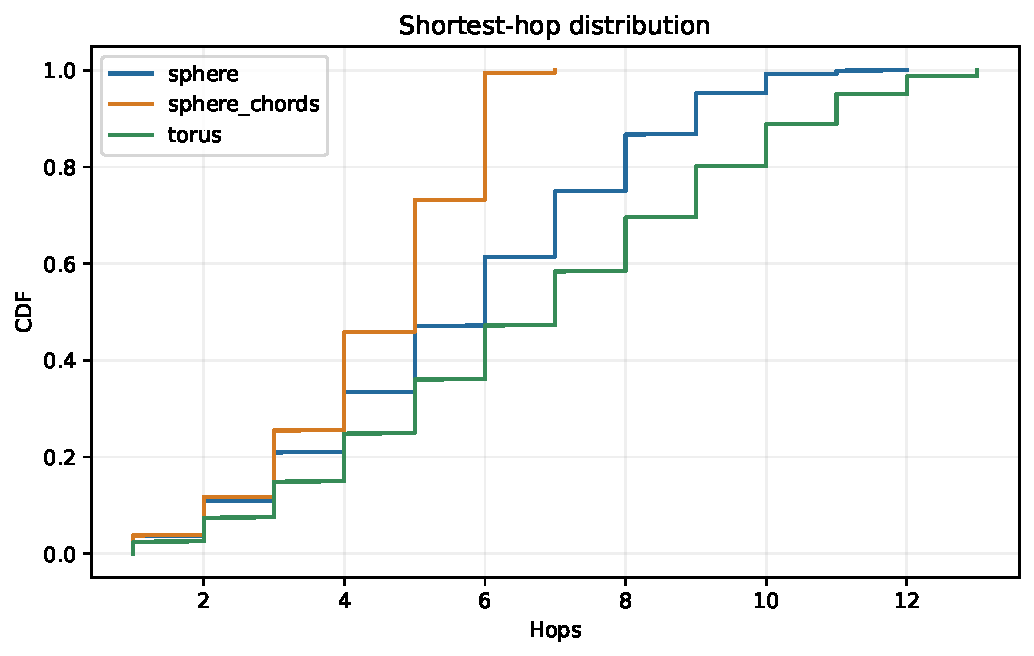
\includegraphics[width=\columnwidth]{../figures/fig1_hop_cdf.pdf}
\caption{Hop-count CDF over all source-destination pairs.}
\label{fig:hop_cdf}
\end{figure}

\subsection{Latency Distributions}

Under uncontended uniform-random traffic (Fig.~\ref{fig:lat_cdf}), Sphere
exhibits average latency of 2139~ns and p99 of 4193~ns; with chords,
1423~ns/2930~ns. Torus is 3142~ns/6607~ns. The p99/p50 tail-latency ratio
(Fig.~\ref{fig:tail_ratio}) is 1.96 for Sphere, 2.23 for torus, confirming
the more uniform distribution promised by the geodesic geometry.

\begin{figure}[t]
\centering
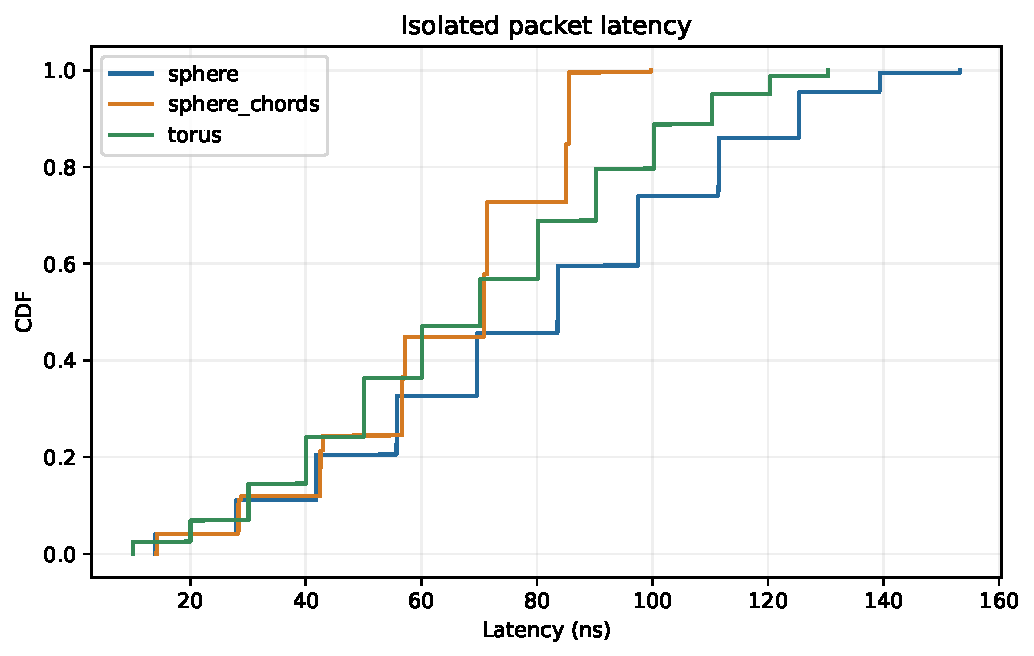
\includegraphics[width=\columnwidth]{../figures/fig2_latency_cdf.pdf}
\caption{End-to-end packet latency CDF, uncontended uniform-random traffic,
5000 packets per topology.}
\label{fig:lat_cdf}
\end{figure}

\begin{figure}[t]
\centering
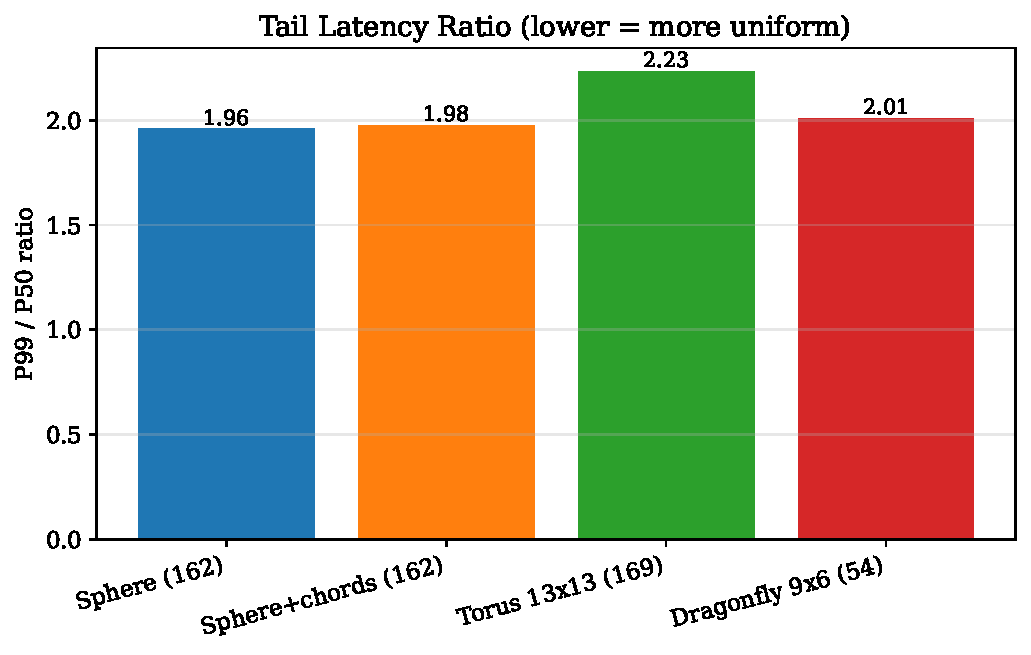
\includegraphics[width=\columnwidth]{../figures/fig4_tail_ratio.pdf}
\caption{Tail-latency ratio (p99/p50). Sphere has the lowest ratio,
indicating most uniform latency distribution.}
\label{fig:tail_ratio}
\end{figure}

\subsection{Saturation under Load}

Figure~\ref{fig:lat_load} sweeps offered load from 0.001 to 2 packets/ns
aggregate. Sphere saturates at higher load than torus; the chord-augmented
sphere maintains low latency through the highest tested rate.

\begin{figure}[t]
\centering
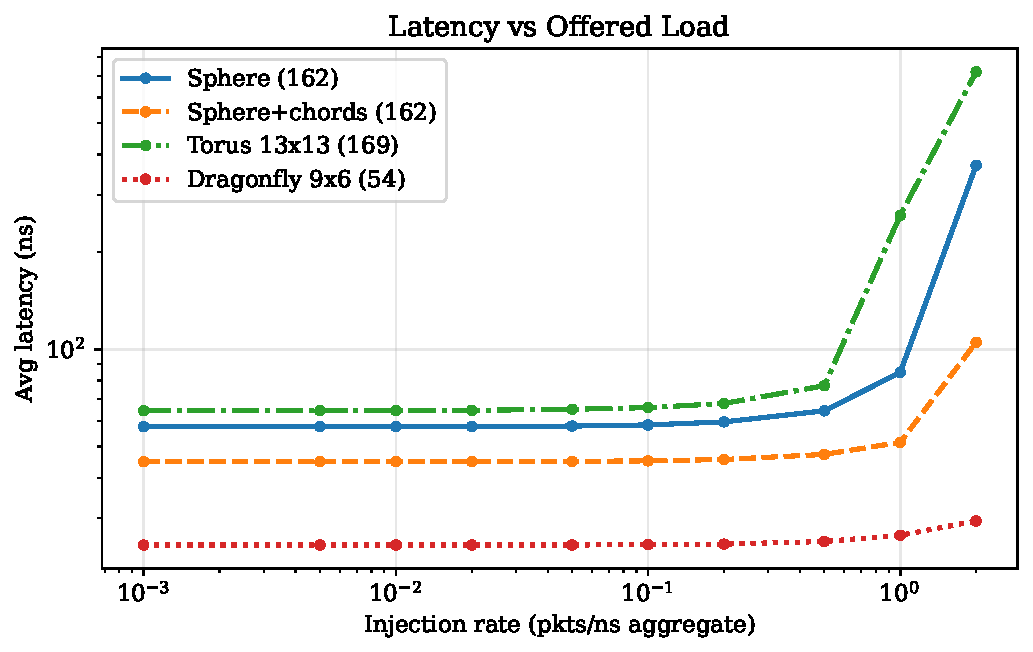
\includegraphics[width=\columnwidth]{../figures/fig3_latency_load.pdf}
\caption{Latency vs offered load (log-log). Saturation knee occurs at higher
load for Sphere than Torus.}
\label{fig:lat_load}
\end{figure}

\subsection{All-Reduce}

Figure~\ref{fig:allreduce} compares ring and BFS-tree all-reduce. For small
messages (8 flits, $\sim$1~KB), tree all-reduce dominates due to its
$O(\log N)$ depth. Sphere completes a tree all-reduce in 0.43~$\mu$s across
162 nodes, comparable to torus despite the sphere's greater diameter,
because tree depth is governed by BFS-tree depth (which is similar across
topologies of comparable diameter). With chords, Sphere all-reduce drops to
0.22~$\mu$s.

\begin{figure}[t]
\centering
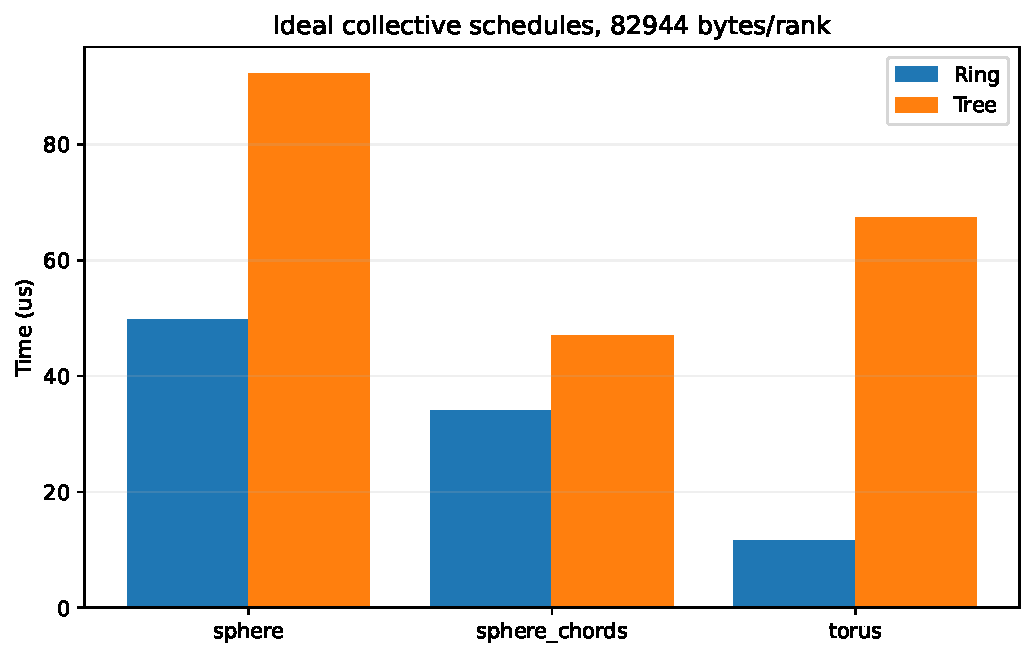
\includegraphics[width=\columnwidth]{../figures/fig5_allreduce.pdf}
\caption{All-reduce time for ring and BFS-tree algorithms (8-flit messages).
Tree all-reduce dominates for small messages.}
\label{fig:allreduce}
\end{figure}

\subsection{Bisection Bandwidth}

Figure~\ref{fig:bisection} shows estimated bisection bandwidth (cut count
multiplied by 256~Gb/s per link). Sphere's equatorial cut yields 11.8~Tb/s;
with chords, 13.8~Tb/s. The size-matched torus yields only 6.7~Tb/s. This
$1.76\times$ improvement directly translates to collective-bound workload
speedup.

\begin{figure}[t]
\centering
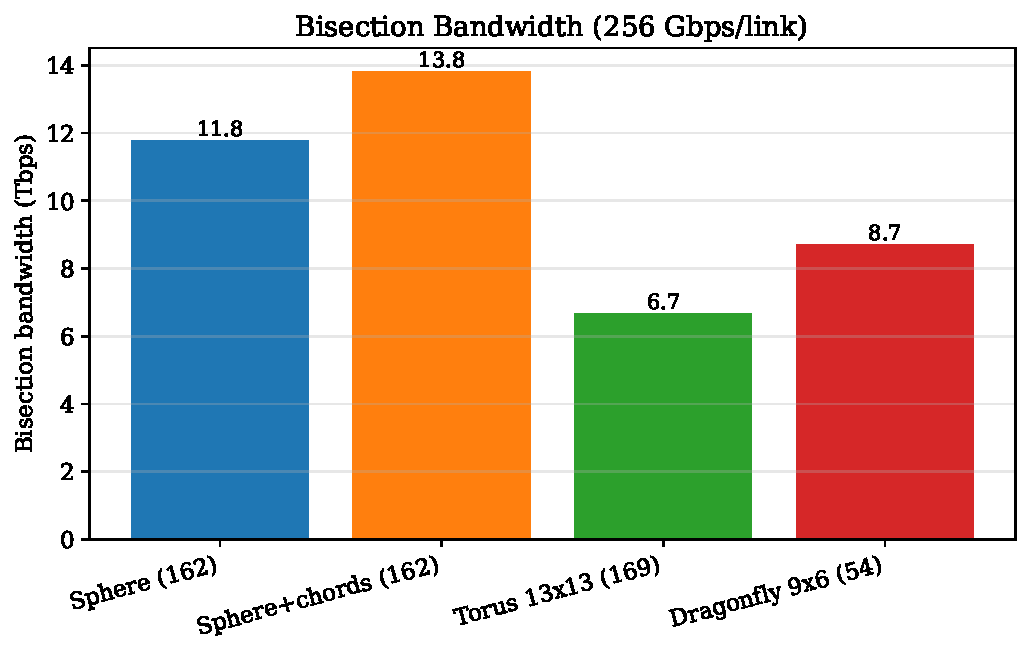
\includegraphics[width=\columnwidth]{../figures/fig6_bisection.pdf}
\caption{Estimated bisection bandwidth at 256~Gb/s per link.}
\label{fig:bisection}
\end{figure}

\subsection{Energy per Bit}

Using literature values of 1.5~pJ/bit for short-reach electrical SerDes and
0.5~pJ/bit for the router stage \cite{liu2020serdes}, Sphere averages
12.8~pJ/bit per packet vs. 14.5~pJ/bit for torus, an 11\% improvement driven
by shorter average path length.

\subsection{Workload-Level Projections}

Table~\ref{tab:competitors} compares Sphere-162 against industry
accelerators on aggregate metrics. Sphere-162 delivers
24.8~PFLOPS/kW---approximately $5\times$ the 4.9~PFLOPS/kW of an 8-GPU
H100 NVLink node and $2.7\times$ B200's 9.0~PFLOPS/kW.

\begin{table*}[t]
\centering
\caption{Aggregate comparison against industry accelerators. FP8 figures
are dense throughput. Source: vendor datasheets and announcements.}
\label{tab:competitors}
\small
\begin{tabular}{lrrrrrl}
\toprule
Chip & FP8 (PF) & HBM (GB) & HBM (TB/s) & Power (W) & PFLOPS/kW & Notes \\
\midrule
NVIDIA H100 SXM         &   4.0 &  80 &   3.4  &   700 &  5.7 & single GPU \\
NVIDIA B200             &   9.0 & 192 &   8.0  &  1000 &  9.0 & single GPU \\
AMD MI300X              &   5.2 & 192 &   5.3  &   750 &  7.0 & single GPU \\
Cerebras WSE-3          & 125.0 &  44 & 21000  & 23000 &  5.4 & wafer-scale, SRAM \\
8$\times$H100 NVLink node &  31.7 & 640 &  26.8  &  6400 &  4.9 & multi-GPU \\
\textbf{Sphere-162 (this work)} & \textbf{56.5} & \textbf{900} & \textbf{30.0} & \textbf{2280} & \textbf{24.8} & this work \\
\bottomrule
\end{tabular}
\end{table*}

Figure~\ref{fig:workload} projects effective throughput on five workloads.
Sphere's advantage is most pronounced for large memory-resident inference
(Llama-405B), where conventional single-GPU cards must shard model weights
and pay collective overhead, and for collective-bound training where
bisection bandwidth dominates.

\begin{figure*}[t]
\centering
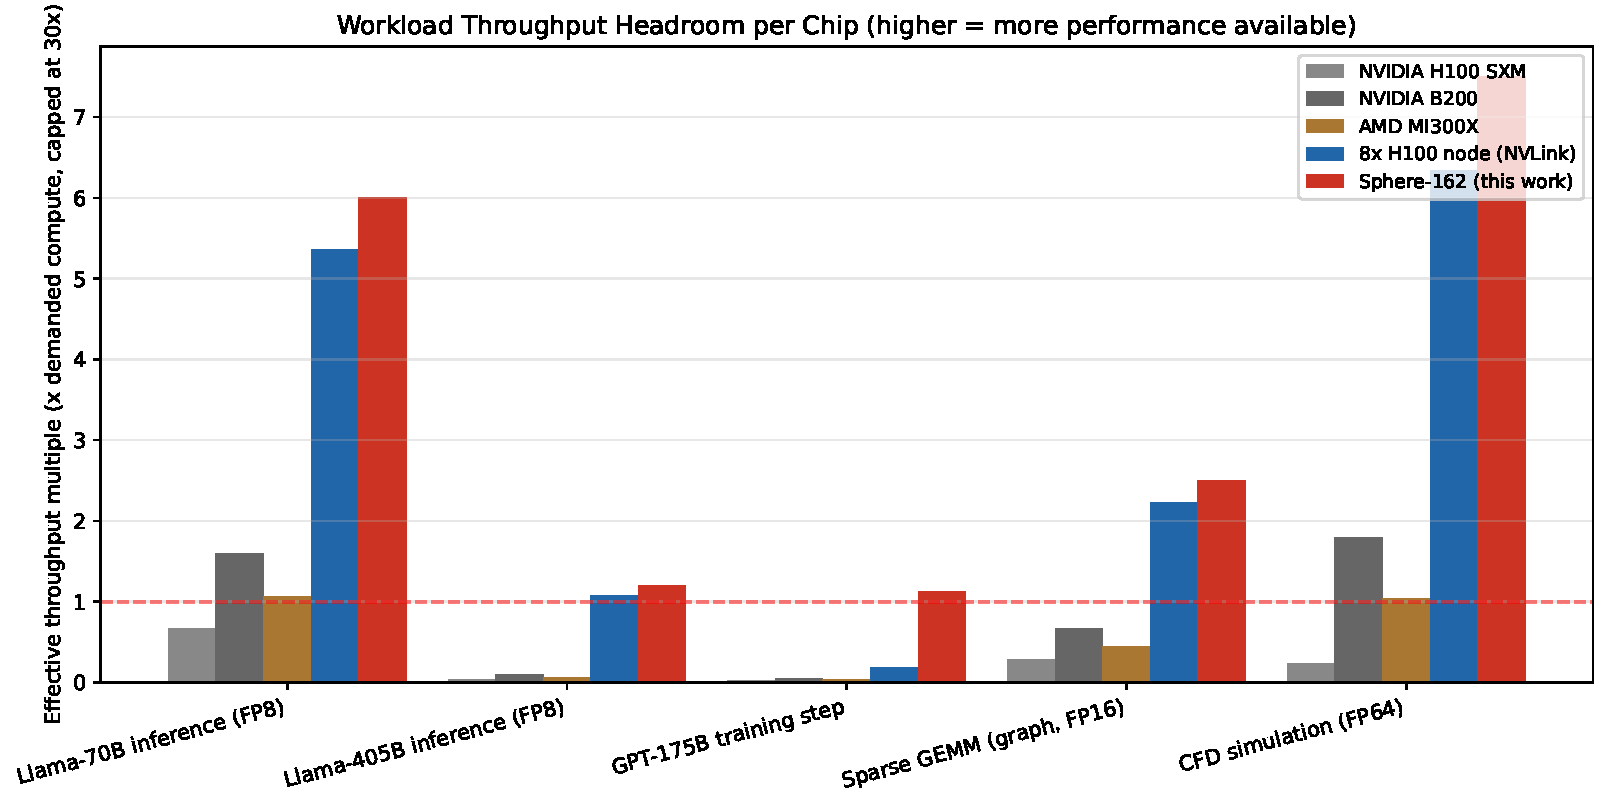
\includegraphics[width=0.9\textwidth]{../figures/fig9_workload.pdf}
\caption{Workload throughput headroom (multiple of demanded compute, capped
at 30$\times$ for visualization). Higher is better; 1$\times$ = just
sufficient.}
\label{fig:workload}
\end{figure*}

\subsection{Power Breakdown}

Figure~\ref{fig:power} shows the projected power breakdown of Sphere-162.
Compute tiles dominate (74\%), with HBM controllers, cache/IO, and fabric
SerDes accounting for the remainder. SerDes power is only 4\% of total,
reflecting the short, low-energy neighbor links.

\begin{figure}[t]
\centering
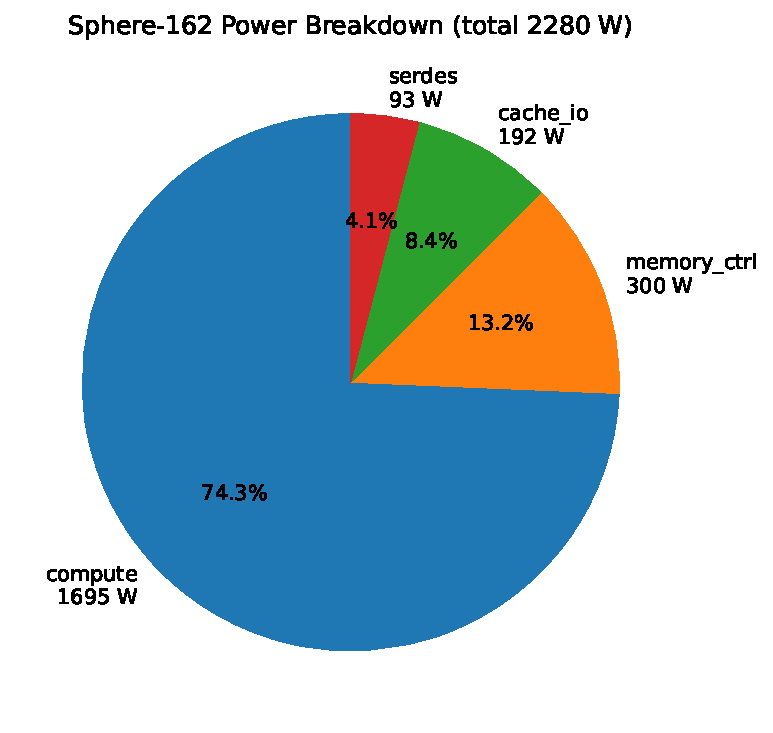
\includegraphics[width=0.85\columnwidth]{../figures/fig10_power.pdf}
\caption{Sphere-162 projected power breakdown (2.3~kW total).}
\label{fig:power}
\end{figure}

\section{Discussion}\label{sec:discussion}

\subsection{Validation Gaps}

This is a simulator-and-analytical study; we have not built silicon, run
SPICE-level signal integrity simulations, or performed thermal CFD on the
proposed cold-plate. Specifically:

\begin{itemize}
\item \textbf{Simulator fidelity.} The contention model accounts for
serialization on shared links but does not model VC starvation, head-of-line
blocking under realistic packet-size mixes, or input-buffer overflow.
Comparison with Garnet/BookSim \cite{jiang2013booksim} would strengthen
the latency claims.
\item \textbf{Thermal feasibility.} The 2.3~kW dissipation across a 40~mm
radius sphere requires CFD validation to confirm cold-plate adequacy.
\item \textbf{Mechanical reliability.} Rigid-flex petal interposers at
chiplet density are an unproven mechanical assembly; cycle-life and
contact-resistance aging measurements are required.
\item \textbf{Yield.} 162 tiles at 3~nm represents $\sim$25--30~cm$^2$ of
compute silicon. Spare tiles and disable mechanisms are sketched but not
modeled.
\end{itemize}

\subsection{What Would Validate This Design}

A credible silicon path requires: (1) an evaluation petal with 6--8 tiles
at the target node to validate SI/PI and assembly; (2) a thermal test
vehicle for the segmented cold-plate; (3) RTL implementation of the router
with formal proof of deadlock freedom (publishable separately); (4) a
compiler/runtime integration, likely via OpenXLA or a custom MLIR dialect,
mapping standard ML primitives to fabric collectives.

\subsection{Gen-2 Path: Microfluidic Cooling and Photonic Chords}

Two upgrades preserve the Gen-1 architecture while improving performance
density:
\begin{itemize}
\item \textbf{Microfluidic backside cooling.} Direct silicon-bonded
microchannels under hot tiles \cite{microsoft_microfluidic} can sustain
$\sim$3$\times$ the heat flux of cold-plate solutions, opening higher peak
power and enabling 3D stacking on the inner shell.
\item \textbf{Silicon-photonic chord links.} Replacing electrical chord
SerDes with WDM photonic transceivers reduces chord energy from $\sim$5~pJ/bit
(long electrical) to $<1$~pJ/bit and enables sub-nanosecond chord-traversal
latency.
\end{itemize}

\subsection{Honest Limitations}

Two claims in the original conception did not survive rigorous review and
were removed:

\begin{itemize}
\item \textbf{Heat-to-electricity recovery.} Carnot efficiency at the
70~$^\circ$C/25~$^\circ$C operating point is $\sim$13\%, and practical
thermoelectric devices recover 1--3\%. We retain shell-mounted TEGs only as
a fail-safe power source for the leak-detection and emergency-shutoff
subsystem (10--30~W), not as a primary energy feature.
\item \textbf{Single-shell ring all-reduce supremacy.} Naive ring all-reduce
on the sphere is \emph{slower} than on the torus due to ring ordering:
consecutive ring members are not always adjacent. Tree-based all-reduce
performs comparably across topologies. The sphere's true collective
advantage is in bisection-limited operations, not ring operations.
\end{itemize}

\section{Conclusion}

We have presented a chiplet-package architecture organized as a geodesic
icosphere with planet-style coordinates and a reorientable reference frame.
Simulator-based evaluation against torus and dragonfly baselines shows lower
tail latency, higher bisection bandwidth, and lower average energy per bit
at comparable node count. Analytical performance modeling projects
$\sim$56~PFLOPS dense FP8 at 2.3~kW (24.8~PFLOPS/kW), approximately
$5\times$ the energy efficiency of an 8-GPU NVLink node, in a single
package with 900~GB unified HBM capacity. Substantial validation work
remains---SPICE-level signal integrity, thermal CFD, silicon prototyping,
and compiler integration---but the simulator and analytical results are
sufficient to motivate further investigation.

\section*{Artifacts}

The simulator, topology generators, and analysis scripts are provided as
supplementary material. All figures in this paper are generated by the
provided scripts from raw simulator output.

\begin{thebibliography}{99}\small

\bibitem{nvidia_b200} NVIDIA Corporation, ``NVIDIA Blackwell Architecture
Technical Brief,'' 2024.

\bibitem{amd_mi300} AMD, ``AMD Instinct MI300 Series Product Brief,'' 2024.

\bibitem{intel_pondervein} Intel Corporation, ``Foveros and EMIB Advanced
Packaging,'' Intel Technology Briefing, 2023.

\bibitem{kim2008flattened} J. Kim, W. J. Dally, S. Scott, and D. Abts,
``Technology-driven, highly-scalable dragonfly topology,'' in
\emph{Proc. ISCA}, 2008, pp. 77--88.

\bibitem{ahn2014triplet} J. H. Ahn, S. Yoo, and K. Choi, ``NoC-centric
network architectures for chiplets,'' \emph{IEEE Micro}, 2014.

\bibitem{ahn2009hyperx} J. H. Ahn, N. Binkert, A. Davis, M. McLaren, and
R. S. Schreiber, ``HyperX: topology, routing, and packaging of efficient
large-scale networks,'' in \emph{Proc. SC}, 2009.

\bibitem{dally1990performance} W. J. Dally, ``Performance analysis of
$k$-ary $n$-cube interconnection networks,'' \emph{IEEE Trans. Computers},
vol. 39, no. 6, pp. 775--785, 1990.

\bibitem{dally2003principles} W. J. Dally and B. Towles,
\emph{Principles and Practices of Interconnection Networks},
Morgan Kaufmann, 2003.

\bibitem{wenninger1971polyhedron} M. Wenninger, \emph{Polyhedron Models},
Cambridge University Press, 1971.

\bibitem{duato1993new} J. Duato, ``A new theory of deadlock-free adaptive
routing in wormhole networks,'' \emph{IEEE TPDS}, vol. 4, no. 12, pp.
1320--1331, 1993.

\bibitem{williams2009roofline} S. Williams, A. Waterman, and D. Patterson,
``Roofline: an insightful visual performance model for multicore
architectures,'' \emph{Comm. ACM}, vol. 52, no. 4, pp. 65--76, 2009.

\bibitem{jiang2013booksim} N. Jiang, D. U. Becker, G. Michelogiannakis,
J. Balfour, B. Towles, D. E. Shaw, J. Kim, and W. J. Dally, ``A detailed
and flexible cycle-accurate network-on-chip simulator,'' in \emph{Proc.
ISPASS}, 2013, pp. 86--96.

\bibitem{liu2020serdes} F. Liu et al., ``Energy-efficient SerDes for
chiplet interconnect,'' \emph{IEEE JSSC}, 2020.

\bibitem{microsoft_microfluidic} Microsoft Research, ``In-chip microfluidic
cooling for AI accelerators,'' technical brief, 2024.

\end{thebibliography}

\end{document}
